% (c) 2015 Daniele Zambelli daniele.zambelli@gmail.com
% (c) 2016 Andrea Sellaroli andrea.sellaroli@istruzione.it

\chapter{Matematica finanziaria}

\begin{comment}
Scambi M-M', M-D-M', D-M-D' e D-D'
\end{comment}

La matematica finanziaria è quella parte della matematica applicata che si 
occupa degli scambi di somme di denaro disponibili in tempi diversi.

Se presto una certa somma di denaro (\textbf{capitale}) per un anno, io non 
potrò più usare quel denaro, e mi aspetto di essere remunerato per ciò. 
Specularmente, se uso del denaro che non possiedo, dovrò pagare una certa somma 
per il prestito ricevuto. 

L'\textbf{interesse} è il compenso che spetta a colui che concede in prestito 
un capitale, rinunciando per un certo periodo di tempo al suo utilizzo. Il 
capitale prestato è detto iniziale, e la percentuale dell'iniziale che va 
pagata annualmente come interesse è detta tasso di interesse. L'usura è la 
pratica consistente nel fornire prestiti a tassi di interesse esorbitanti in 
modo da rendere il loro rimborso difficile o addirittura impossibile, spingendo 
perciò il debitore ad accettare condizioni sempre più pesanti poste dal 
creditore.

Il \textbf{tasso di interesse} viene espresso come una percentuale per un dato 
periodo di tempo e indica quanta parte della somma prestata debba essere 
corrisposta come interesse al termine del tempo considerato o, da un altro 
punto di vista, indica il costo del denaro. Il debitore, infatti, ricevendo una 
somma di denaro, si impegna a pagare una somma superiore a quella ricevuta. La 
differenza costituisce l'interesse, che viene solitamente calcolato in 
percentuale sulla somma prestata.

\begin{exrig}
\begin{esempio}
Deposito in banca 3000 € \,e, un anno dopo, ne ritiro 3150 €. Gli interessi sono 
dati dalla differenza tra il capitale finale e il capitale iniziale e quindi 
sono 150 €. Il tasso di interesse è la percentuale degli interessi sul capitale 
iniziale e quindi
$$ i = \dfrac{150}{3000} = 0,05 $$
ovvero il 5\%. \`{E} importante notare che tale tasso di interesse è 
strettamente riferito al periodo di tempo (in questo caso un anno). Pertanto è 
più corretto affermare che il tasso di interesse è del 5\% annuo. 
\end{esempio}

\begin{esempio}
Ho acquistato un nuovo computer di 700 € sfruttando un offerta che mi permette 
di pagarlo tra un anno, pagando un interesse del 3\%.
L'interesse che dovrò pagare sarà di $700 \cdot 0,03 = 21$ € ed alla fine il 
computer mi costerà 721 €
\end{esempio}

\end{exrig}

Oltre che dalla percentuale, i tassi d'interesse sono caratterizzati dal 
cosiddetto regime di capitalizzazione degli interessi, che può essere semplice 
o composto. Se la durata del prestito è superiore al periodo di tempo per cui 
l'interesse viene conteggiato, si parla di tasso di interesse composto, perché 
vengono conteggiati nel calcolo dell'interesse finale anche gli interessi 
parziali già maturati per ogni periodo.

\section{Interesse semplice}
L'interesse viene detto semplice quando è proporzionale al capitale e al tempo. 
Ovvero gli interessi, maturati da un dato capitale nel periodo di tempo 
considerato, non vengono aggiunti al capitale che li ha prodotti 
(capitalizzazione) e, quindi, non maturano a loro volta interessi. Indichiamo:

\begin{itemize}
\item \textbf{C} il capitale iniziale;
\item \textbf{i} il tasso di interesse periodale (in genere tasso unitario annuo, ma 
può essere mensile, trimestrale...);
\item \textbf{t} durata temporale dell'operazione, espressa in numero di periodi (in 
genere anni);
\item \textbf{M} il capitale finale, detto anche montante, pari alla somma di capitale 
iniziale più gli interessi maturati. 
\end{itemize}

All'istante iniziale ($t=0$) possiamo dire che il montante coincide col 
capitale $$ M_{0}=C $$
Dopo un periodo di tempo ($t=1$), il montante sarà dato dal capitale più 
l'interesse. 
$$ M_{1}=M_{0} +iC = C + iC $$
Analogamente dopo 2, 3 e 4 periodi di tempo il capitale sarà dato da 
$$ M_{2}=M_{1} +iC = (C + iC) +iC = C +2iC$$
$$ M_{3}=M_{2} +iC = (C + 2iC) +iC = C +3iC$$
$$ M_{4}=M_{3} +iC = (C + 3iC) +iC = C +4iC$$
In generale possiamo calcolare il montante per il periodo successivo con la 
formula:
$$ M_{t}=M_{t-1}+iC=C(1+t\cdot i) $$
\begin{definizione}[Capitalizzazione semplice]
$$ M_{t}=C(1+t\cdot i) $$
\end{definizione}

\begin{exrig}
\begin{esempio}
Una persona deposita 5000 € in banca al tasso di interesse annuo del 5\%. Dopo 
4 anni preleva la somma e la reinveste al tasso annuo del 6\%. Dopo altri 5 
anni 
e 9 mesi di che cifra dispone?
Il capitale iniziale è di 5000 € ed applicando la formula di capitalizzazione 
semplice otteniamo che il montante dopo 4 anni è

$$M_4 = 5000(1+4\cdot0,05) = 6000$$
Quando questa cifra viene prelevata e reinvestita possiamo considerarla come il 
un nuovo capitale iniziale. La durata temporale, in questo caso, è espressa in 
anni e in mesi. Convertendola in anni otteniamo $t = 5 +\frac{9}{12} = 5,75$ e 
quindi

$$M_{5,75} = 6000(1+5,75\cdot0,06) = 8070$$
\end{esempio}
\end{exrig}

\section{Interesse composto}

L'interesse viene detto composto quando, invece di essere pagato o riscosso, è 
aggiunto al capitale iniziale che lo ha prodotto. Questo comporta che, alla 
maturazione degli interessi, il montante verrà riutilizzato come capitale 
iniziale per il periodo successivo. Quindi anche l'interesse stesso produce a sua volta interesse.

In questo caso quindi gli interessi si sommano al capitale iniziale che li ha 
prodotti al termine di ogni periodo.
Analogamente a prima il montante iniziale coincide col capitale
$$ M_{0}=C $$
Dopo un periodo il montante sarà dato dal capitale più l'interesse
$$M_{1}=C+iC=C(1+i)$$
Calcoliamo adesso l'interesse su tutto il montante $M_1$ e troviamo
$$M_{2}=M_1+iM_1=M_1(1+i)=C(1+i)^2$$
$$M_{3}=M_2+iM_2=M_2(1+i)=C(1+i)^3$$
ed in generale risulta
$$M_{t}=M_{t-1}(1+i) = C(1+i)^{t-1}(1+i)=C(1+i)^{t}$$

\begin{definizione}[Capitalizzazione composta]
$$ M_{t}=C(1+i)^t $$
\end{definizione}

In generale il periodo considerato è l'anno. Spesso però vengono considerati 
anche gli interessi che maturano $t$ volte durante l'anno, ma sempre in periodi 
definiti. In genere viene definito un tasso annuo nominale $i$ al quale 
corrisponde un tasso convertibile $i_c$ dato da

$\ i_c = \frac{i}{t}$.

Per il calcolo del montante si applica la stessa formula impiegata per 
l'interesse composto
$\ M_n = C (1+i_c)^{nt} = C \left(1+\frac{i}{t}\right)^{nt}$.

dove $i_c$ è l'interesse convertibile e $nt$ indica il numero di volte in cui 
l'interesse convertibile matura nell'intero periodo.

\begin{exrig}
\begin{esempio}
Un ``amico'', 20 anni fa, mi ha prestato 500 € al tasso di interesse del 9\% in 
regime di capitalizzazione composta. Per capire quanto gli devo restituire oggi 
posso usare la formula per la capitalizzazione composta.
$$M_{20} = 500(1+0,09)^{20} = 2802,21$$ 
Come si nota subito in 20 anni la cifra iniziale è più che quintuplicata. In 
effetti il tasso del 9 \% è un tasso da usura. 
\end{esempio}
\begin{esempio}
Un capitale di 10000 € è stato investito per un periodi di 30 mesi al tasso 
trimestrale convertibile dell'1\% . Considerando che ci sono 4 trimestri in un 
anno, il tasso annuo nominale risulta quindi
$$i=i_c\cdot t=1\cdot 4=4\%$$
Dopo 30 mesi, ovvero 10 trimestri, il montante risulta
$$M=10000(1+0,01)^{10}=11046,22$$
\end{esempio}
\end{exrig}

\section{Capitalizzazione composta continua}

In questo caso gli interessi si sommano al capitale che li ha prodotti ad ogni 
istante. Il tasso d'interesse composto a capitalizzazione continua ha 
applicazioni soprattutto teoriche, nella matematica finanziaria; sebbene sia 
rilevante nelle applicazioni relative alle più semplici operazioni finanziarie, 
è ad esempio ampiamente utilizzato nelle formule di valutazione di operazioni 
finanziarie complesse, come nella valutazione delle opzioni.

L'interesse in capitalizzazione continua può essere giustificato come segue. Si 
consideri un tasso annuale $i$, e si supponga di suddividere l'anno in $t$ 
periodi, al termine di ciascuno dei quali viene corrisposta una frazione 
dell'interesse relativo all'intero anno pari a $\frac{i}{t}$, che viene 
immediatamente reinvestita. A partire da un capitale iniziale $C$, il montante 
al termine di $n$ anni sarà allora
\\[4pt]
$\ M_n=C\left(1+\frac{i}{t}\right)^{nt}$
\\[4pt]
Passando al limite per $t$ che tende a infinito, si ha il caso in cui un flusso 
continuo di pagamenti viene reinvestito in maniera continua; il montante sarà 
dato da
\\[4pt]
$$\ M_n = \lim_{t\to\infty} C\left(1+\frac{i}{t}\right)^{nt} = Ce^{in}$$,
\\[4pt]
ricorrendo al limite notevole che definisce il numero di Nepero $e$.

\subsection{Tassi equivalenti}

Chiamiamo \emph{tassi equivalenti} due tassi d'interesse che, applicati allo stesso capitale,
producono lo stesso montante (ovviamente in tempi diversi).
Per determinare la relazione tra due tassi unitari ad interesse composto 
$i_{c1}$ e $i_{c2}$ è sufficiente uguagliare i montanti che sono prodotti da 
periodi di tempo $t_1$ e $t_2$ differenti
$$M = C(1+i_{c1})^{t_1} = C(1+i_{c2})^{t_2}$$.
Da questa si ottengono le relazioni:
$$i_{c1} = (1+i_{c2})^\frac{t_2}{t_1}-1 \hspace{1cm} i_{c2} = (1+i_{c1})^\frac{t_1}{t_2}-1$$



\section{Rendite}
Una rendita finanziaria è una successione di importi, chiamate rate, da 
riscuotere (o da pagare) in epoche differenti, chiamate scadenze, ad intervalli 
di tempo determinati. 

Una rendita S è quindi individuata da 3 argomenti:

\begin {itemize}[noitemsep]
\item $R_k\;$ : rata da riscuotere (o da pagare) alla scadenza $t_k\;$
\item $t_k\;$ : scadenza, cioè il momento all'interno del k-esimo intervallo in 
cui viene riscossa (o pagata) la rata $R_k\;$
\item $n\;$: numero di rate totali
\end{itemize}

e si può indicare con $ S= ( R_k , \; t_k\;)$  dove $ k \;=0,1,2,...,n$
\\[4pt]
Ci occuperemo nel seguito di un tipo di rendite particolarmente semplice:
il numero delle rate totali è finito e le scadenze sono separate da intervalli 
di tempo uguale. La prima rata viene riscossa (o pagata) 
al termine del primo intervallo. Tale tipologia di rendita viene detta \emph{rendita 
periodica posticipata immediata}.

\begin{figure}[htp]
\centering
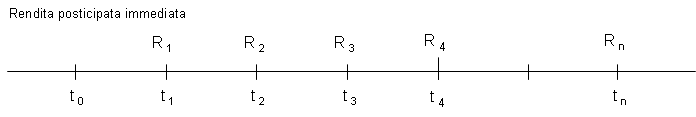
\includegraphics[scale=.60]{img/rendite.png}
\caption{}
\label{}
\end{figure}

\subsection{Valore attuale delle rendite}
Il valore attuale di una rendita è il valore $V(t_0)$  calcolato al tempo $t = 
t_0$  ed equivale alla somma dei valori attuali delle singole rate della 
rendita nel regime di capitalizzazione prescelto.

Il valore $V(t_j)$ di una rendita finanziaria all'istante $t_j$ è la somma dei valori
attuali delle rate con scadenze antecedenti a $t_j$, dei valori attuali delle rate con 
scadenze successive a $\;t_j$, ed eventualmente della rata $\;R_j$ con scadenza 
$\;t_j$.

\subsubsection{Rendita posticipata}

Nel caso di una rendita periodica posticipata immediata di n rate costanti, nel 
regime di sconto composto per un periodo \(\; p= 
t_{k+1}-t_k\), con tasso di interesse $i$, il fattore di sconto per un periodo p è:
\[g(t_k-t_0)=\frac{1}{(1+i)^k} \qquad \text{e quindi:} \quad \; V(t_0)=\sum^{n}_{k=0}R_k \; g(t_k\;-\;t_0)= \; \sum^{n}_{k=0}R_k \; 
\frac{1}{(1+i)^k}\]
essendo la rendita posticipata immediata e a rata costante: $\;R_{0}=0 \quad$ e 
$\;R_{1}=R_{2}=...=R_{n}=R$:
\[\begin{aligned}
   V(t_0)&=\; \sum^{n}_{k=0}R_k \; \frac{1}{(1+i)^k} =\cancel{R_0 \; 
\frac{1}{(1+i)^0}}+R_1 \; 
\frac{1}{(1+i)^1}+\dots+R_n \; 
\frac{1}{(1+i)^n} =\\
&= R\; 
\frac{1}{(1+i)^1}+\dots+R \; 
\frac{1}{(1+i)^n} = R\; \quadra{
\frac{1}{(1+i)^1}+\dots+\; 
\frac{1}{(1+i)^n}} = R \sum^{n}_{k=1}\tonda{\frac{1}{1+i}}^k 
  \end{aligned}
\]
Consideriamo per un attimo solamente la somma: ricordando la formula per le somme parziali di una serie geometrica
\footnote{Data una serie geometrica di ragione $v$ si dimostra che: 
\(\displaystyle \sum^{n}_{k=1} v = v\; \frac{1-v^n}{1-v}\)} ed osservando che, nel nostro caso, la ragione
della serie vale $v = \tonda{\frac{1}{1+i}}$, si ha:
$$\sum^{n}_{k=1}\tonda{\frac{1}{1+i}}^k = \tonda{\frac{1}{1+i}} 
\;\frac{1-\tonda{\frac{1}{1+i}} ^n}{1-\tonda{\frac{1}{1+i}} }\; = \;\; 
\frac{1-\tonda{\frac{1}{1+i}} ^n}{i} = \frac{1-\tonda{1+i} ^{-n}}{i} =: a_{n^\urcorner i}$$
Definendo questo oggetto come $a_{n^\urcorner i}$ (da 
leggersi ``a posticipato, figurato n, al tasso i''), la formula per $V(t_0)$ diventa:
$$\; V(t_0)= R\cdot\frac{1-(1+i)^{-n}}{i}= R\cdot a_{n^\urcorner i}$$

\subsubsection{Rendita anticipata}

\subsection{Montante delle rendite}
Il montante di una rendita è il valore $\;V(t_n)$ calcolato al tempo $\;t=t_n$ 
ed equivale alla somma dei montanti delle singole rate calcolati al termine 
della rendita nel regime di capitalizzazione prescelto.


Nel caso del montante di una rendita periodica anticipata immediata di n rate, 
nel regime a interesse composto per un periodo 
$p= t_{k+1}-t_k$, con tasso d'interesse $\;i$, il fattore di montante è
$$f(t_n-t_k)=(1+i)^{n-k} \qquad \text{e quindi:} \quad V(t_n)=\; \sum^{n}_{k=0}R_k\; f(t_n\;-\;t_k)= \; \sum^{n}_{k=0}R_k\; 
(1+i)^{n-k}$$
essendo la rendita anticipata immediata (e a rata costante) l'ultima rata viene 
pagata all'istante $t_{n-1}$ e quindi $\;R_n=0$, e 
$\;R_{0}=R_{1}=R_{2}=...=R_{n-1}=R$
$$\begin{aligned}
   V(t_n)&=\; \sum^{n}_{k=0}R_k\; 
(1+i)^{n-k}= R_0\; 
(1+i)^{n}+\dots+R_{n-1}\; 
(1+i)^{1}+\cancel{R_n\; 
(1+i)^{0}}\\
&=R\; 
(1+i)^{n}+\dots + R\; 
(1+i)= \;R \;\left[(1+i)^n+\dots+(1+i)\right]\;=\;R\; 
\sum^{n}_{k=1}\; (1+i)^{k}
  \end{aligned}
$$
Come sopra, consideriamo solamente la somma. In questo caso la ragione
della serie vale $v = \tonda{1+i}$, perciò:
$$\sum^{n}_{k=1}\; (1+i)^{k} =\tonda{1+i} \frac{1-\tonda{1+i}^n}{1-\tonda{1+i}}=
\frac{(1+i)[(1+i)^{n}-1]}{i}=:\ddot{s}_{n^\urcorner i}$$
quindi il montante $\; V(t_n)$ di una generica rendita di $\;n$ rate $\;R$ 
costanti e anticipate si può scrivere:
$$\; V(t_n) = R\cdot\frac{(1+i)[(1+i)^{n}-1]}{i} = R\cdot\ddot{s}_{n^\urcorner 
i}$$
Nel caso di una rendita (sempre periodica e unitaria) con pagamenti posticipati il montante sarà dato invece da:
$$\; V(t_n)= R\cdot\frac{(1+i)^{n}-1}{i}= R\cdot s_{n^\urcorner i} \qquad \text{dove} \quad
s_{n^\urcorner i} = \frac{(1+i)^{n}-1}{i}$$



